\chapter{Instalação/Configuração da aplicação na Google Cloud}
De seguida apresenta-se o processo de instalação e configuração dos componentes da aplicação, onde foram utilizadas as ferramentas: \textbf{Docker}, \textbf{Kubernetes}. 

\section{Vantagens da utilização de Containers}
A utilização de containers na infraestrutura da aplicação \textbf{zulip}, permite um isolamento dos componentes, bem como um melhor aproveitamento dos recursos de cada máquina, facilitando o processo de teste, \emph{provisining} e migração dos mesmos, sendo estes importantes num processo de \textsf{deployment}.

\section{Abordagens}
Com uma análise da arquitetura da aplicação \textbf{Zulip}, percebeu-se a existência de pontos críticos (\textbf{SPOFS}).\newline Na verdade, não se deve conter num sistema componentes únicos, que em sua falta, causem a falha de todo o sistema. \newline Assim, para uma redução da probabilidade de acontecimento destes, achou-se que a solução seria a replicação dos componentes onde estes acontecem.
Operações que façam acessos à base dados, ou apenas ao servidor aplicacional, estão dependentes destes componentes, sendo crucial a fiablidade dos mesmos.
Assim, todos os componentes devem ser replicados, excepto o \textbf{NGINX}, visto a impossibilidade de replicação deste.\newline
A replicação destes componentes também contribuí para uma melhor disponibilidade, visto que, há uma distribuiçao de carga pelas várias réplicas.

\section{Docker}
A ferramenta \textbf{Docker} consiste numa plataforma para \emph{developers}, com o objetivo de construir, partihar e executar aplicações com \emph{containers}. O uso desta ferramenta facilita o processo de \textbf{deployment}.\newline As grandes vantagens do \textbf{Docker} são: 
\begin{itemize}
    \item Flexibilidade: a complexidade da aplicação não impede a possibilidade de ser colocada num container;
    \item Leves/eficientes: os recursos e kernel da máquina são partilhados por todos os containers, havendo um melhor aproveitamento dos recursos;
    \item Portabilidade: pode ser construído localmente e fazer-se o \emph{deploy} para a cloud facilmente;
    \item Escabilidade: com facilidade, consegue-se aumentar e distribuir as replicas de containers;
    \item etc ...
\end{itemize}{} 

Na figura \ref{img:docker} verifica-se uma das grandes vantagens da ferramenta \textbf{Docker} em relação à utilização de \textbf{VMs} para agregação de diferentes aplicações na mesma máquina. \newline
Tal como já foi referido, na utilização de máquinas virtuais (caso da direita da figura \ref{img:docker}), há uma repetição de sistemas operativos desnecessária para cada aplicação, e deste modo, recursos usados desnecessariamente para estes sistemas opearativos. \newline Por outro lado, no \textbf{Docker}, existe apenas um sistema operativo, partilhado por todas as aplicações, havendo assim, um melhor aproveitamento dos recursos, pois estes sao distribuídos pelos vários containers.



\begin{figure}[h!]
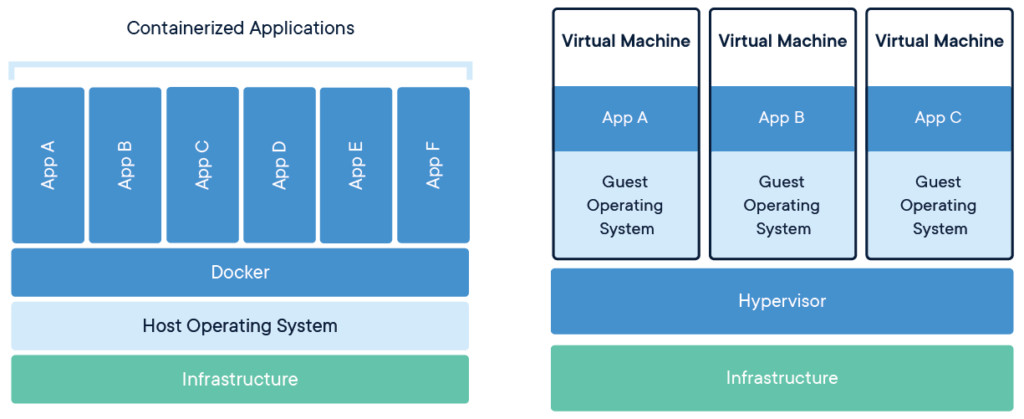
\includegraphics[scale=0.50]{images/docker.png}
\caption{Docker vs VMs.}
\centering
\label{img:docker}
\end{figure}
\newpage

\section{Kubernetes}
Trata-se de uma plataforma de código aberto, que permite gerir aplicações em containeres e automatizar a sua implementação.
\textbf{Kubernetes} introduz o conceito de \textsf{pods} que consiste em um ou mais containers.
Com a utilização do \textbf{Kubernetes}, obtem-se um \textsf{cluster}. Um cluster é um conjunto de máquinas que correm aplicações em containers, que são geridas pelo \textbf{Kubernetes}. O cluster tem pelo menos um nodo (máquina) \textsf{worker} e um \textsf{master}, sendo que o \textsf{worker} corre os \textsf{pods} que são componentes da aplicação no nosso caso \textbf{Zulip}, e o \textsf{master} gere as máquinas \textsf{worker} e os \textsf{pods} do cluster, de notar que múltiplos nós \textsf{master} permite tolerância a falhas e alta disponibilidade.
Neste caso  decidiu-se utilizar um cluster com um \textsf{master} e quatro máquinas \textsf{worker}.

\begin{figure}[h!]
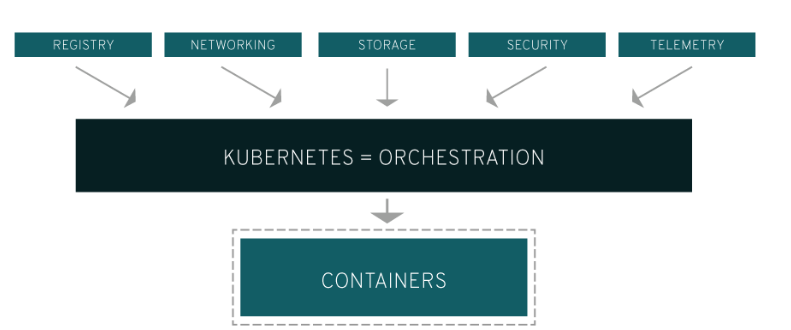
\includegraphics[scale=0.90]{images/kuber.PNG}
\caption{Arquitetura do \textbf{Kubernetes}.}
\centering
\end{figure}

\section{Automatização do Deployment}

A ferramenta \textbf{Kubernetes} facilita bastante a automatização do processo de \textbf{Deployment}, pois consegue-se definir as configurações dos componentes no ficheiro \emph{zulip-rc.yml}, em relação ao número de replicas. Com o ficheiro de configuração preparado, apenas com o comando da figura \ref{img:kub} consegue-se fazer o \textbf{Deployment} para o cluster de \textbf{Kubernetes}, onde automáticamente, os componentes são distribuídos por containers, em diferentes nodos.

\begin{figure}[h!]
\centering
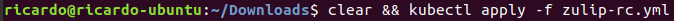
\includegraphics[scale=0.70]{images/5.png}
\caption{Comando automático para \textbf{Deployment}.}
\label{img:kub}
\end{figure}

\begin{figure}[h!]
\centering
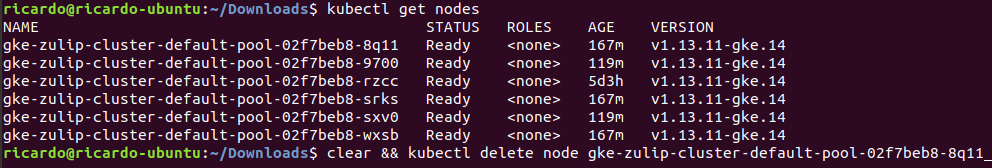
\includegraphics[scale=0.51]{images/3.png}
\caption{Comando de listar nodos, e apagar nodos.}
\end{figure}

\begin{figure}[h!]
\centering
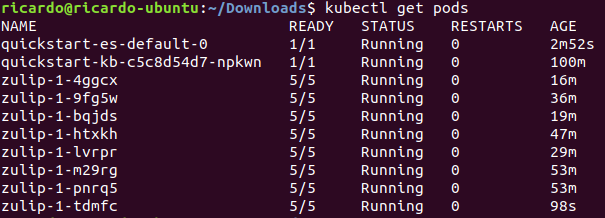
\includegraphics[scale=0.80]{images/2.png}
\caption{Listagem dos \textbf{pods}, replicas dos componentes.}
\end{figure}






\chapter{Monitorização}
As ferramentas utilizadas para Monitorização da infraestrutura foi: \textbf{MetricBeat}, como colecionador e \emph{parser} de dados, \textbf{ElasticSearch}, para analisar (\emph{RESTful search and analytics}) e por fim o \textbf{Kibana}, para visualização dos dados. \newline
Inicialmente, começou-se por criar uma máquina para monitorização, com os componentes \textbf{ElasticSearch} e \textbf{Kibana}, mas ao tentar-se instalar os \textbf{MetricBeats} nos nós do cluster, não se conseguiu. Isto deveu-se ao facto de se estar a usar o \textbf{Kubernetes}, e o mesmo estar preparado para instalar estes componentes de forma automática em containers. \newline 

Apesar da instalação do \textbf{Elasticsearch} e \textbf{Kibana} terem funcionado com \textbf{Kubernetes}, novamente a equipa teve problemas com o \textbf{MetricBeats}, pelo que devido à falta de tempo para conclusão do projeto, decidiu-se usar as métricas de monitorização fornecidas pelo \textbf{Google Cloud}.\newline 

Assim, deste modo, verifica-se que uma das necessidade de métricas, em que a monitorização foi útil, foi a deteção de falta de memória \textbf{RAM}, tal como se pode ver na figura \ref{img:monitorizacao} , quando se testou diferentes configurações dos componentes na fase de \textbf{benchmark}. 

\begin{figure}[h!]
\centering
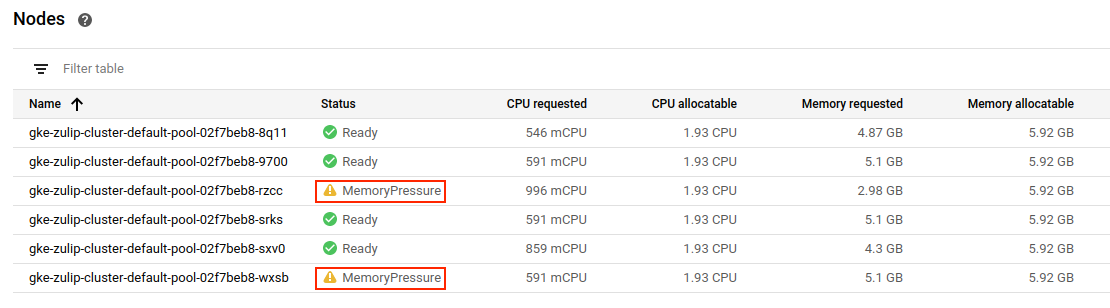
\includegraphics[scale=0.45]{images/monitorizacao.png}
\caption{Monitorização do Google Cloud.}
\label{img:monitorizacao}
\end{figure}

\chapter{Benchmarking}

Após a configuração da arquitetura e deployment do sistema foi efetuado o \textbf{benchmarking} simultâneamente à monitorização, desta forma é possível analisar com \textbf{dados concretos} se a arquitetura atual é \textbf{eficiente} para o uso \textbf{realista} da aplicação zulip por parte de vários clientes. Note-se que não é pretendido ter o sistema com os melhores recursos possíveis, isso seria dispendioso, pretende-se ter recursos suficientes para responder aos pedidos dos clientes atendendo ao binómio \textbf{custo vs rapidez}.
\newline

Foi efetuado 1 \textbf{HTTP(S) request}:

\begin{enumerate}
  \item \label{itm:fst} obtenção página inical: method \textbf{GET} https://zulip/login/
\end{enumerate}

O request foi analisado com o programa \textbf{jmeter} e efetuado com 9 configurações que variam entre o \textbf{número de clientes} e \textbf{número de pedidos de cada cliente} a cada momento. Desta forma os resultados obtidos em relação ao \textbf{número de pedidos por minuto} (throughput)que a aplicação zulip consegue atender e o respetivo tempo total encontram-se nas seguintes tabelas.

\begin{table}[H]
    \centering
    \begin{tabular}{|l||r||r|}
    \hline
        \#Clientes + \#Pedidos & Throughput & Tempo Total\\ \hline \hline
        250 C + 1 P & 65 217 & menos de 1 seg \\ \hline
        250 C + 5 P & 186 567 & menos de 1 seg \\ \hline
        250 C + 10 P & 268 817 & menos de 1 seg \\ \hline
        \hline
        500 C + 1 P & 68 965 & menos de 1 seg \\ \hline
        500 C + 5 P & 72 011 & 2 segs \\ \hline
        500 C + 10 P & 223 665 & 2 seg \\ \hline
        \hline
        1000 C + 1 P & 37 243 & 1 seg \\ \hline
        1000 C + 5 P & 73 511 & 4 segs \\ \hline
        1000 C + 10 P & 180 018 & 5 segs \\ \hline
        
    \end{tabular}
    \caption{Resultados para o HTTP(S) request \ref{itm:fst} (página incial).}
    \label{tab:testeFront}
\end{table}

A topologia final utilizada para estes teste consiste em \textbf{6 nodos} e \textbf{7 réplicas}, note-se que cada réplica utiliza 5 serviços/ containers, logo na realidade a arquitetura consiste em \textbf{6 nodos} e \textbf{35 containers}.

O benchmarking \textbf{foi essencial para otimizar a configuração dos recursos} necessária para o funcionamento fluído da aplicação. 

Inicialmente a configuração era de \textbf{3 nodos} e \textbf{1 réplica} apenas, quando foi analisado HTTP(S) request \ref{itm:fst} verificou-se o seguinte resultado.

\begin{table}[H]
    \centering
    \begin{tabular}{|l||r||r|}
    \hline
        \#Clientes + \#Pedidos & Throughput & Tempo total \\ \hline \hline
        1000 C + 1 P & 457 & 120 segs \\ \hline
    \end{tabular}
    \caption{Resultados para o HTTP(S) request \ref{itm:fst} para \textbf{3 nodos} e \textbf{1 réplica}.}
    \label{tab:testeFront}
\end{table}

Este resultado é péssimo para uma aplicação que à partida é utilizada por muitos clientes simultâneamente, uma vez que uma espera de 2 minutos é impensável, logo foi alterada a topologia, decidiu-se analisar o mesmo HTTP(S) request para várias configurações.

\begin{table}[H]
    \centering
    \begin{tabular}{|l||r||r|}
    \hline
        \#Clientes + \#Pedidos & Throughput & Tempo total \\ \hline \hline
        1000 C + 1 P & 37 428 & 1 seg \\ \hline
    \end{tabular}
    \caption{Resultados para o HTTP(S) request \ref{itm:fst} para \textbf{6 nodos} e \textbf{4 réplicas}.}
    \label{tab:testeFront}
\end{table}

\begin{table}[H]
    \centering
    \begin{tabular}{|l||r||r|}
    \hline
        \#Clientes + \#Pedidos & Throughput & Tempo total \\ \hline \hline
        1000 C + 1 P & 33 783 & 1 seg \\ \hline
    \end{tabular}
    \caption{Resultados para o HTTP(S) request \ref{itm:fst} para \textbf{6 nodos} e \textbf{7 réplicas}.}
    \label{tab:testeFront}
\end{table}

\begin{table}[H]
    \centering
    \begin{tabular}{|l||r||r|}
    \hline
        \#Clientes + \#Pedidos & Throughput & Tempo total \\ \hline \hline
        1000 C + 1 P & 71 942 & menos de 1 seg \\ \hline
    \end{tabular}
    \caption{Resultados para o HTTP(S) request \ref{itm:fst} para \textbf{6 nodos} e \textbf{8 réplicas}.}
    \label{tab:testeFront}
\end{table}

\begin{table}[H]
    \centering
    \begin{tabular}{|l||r||r|}
    \hline
        \#Clientes + \#Pedidos & Throughput & Tempo total \\ \hline \hline
        1000 C + 1 P & 39 040 & 1 seg \\ \hline
    \end{tabular}
    \caption{Resultados para o HTTP(S) request \ref{itm:fst} para \textbf{6 nodos} e \textbf{10 réplicas}.}
    \label{tab:testeFront}
\end{table}

\begin{table}[H]
    \centering
    \begin{tabular}{|l||r||r|}
    \hline
        \#Clientes + \#Pedidos & Throughput & Tempo total \\ \hline \hline
        1000 C + 1 P & 574 & 112 segs \\ \hline
    \end{tabular}
    \caption{Resultados para o HTTP(S) request \ref{itm:fst} para \textbf{8 nodos} e \textbf{8 réplicas}.}
    \label{tab:testeFront}
\end{table}

Conclui-se que a melhor configuração seria \textbf{6 nodos} e \textbf{8 réplicas}, no entanto após algum tempo com a configuração ativa notou-se que por certos períodos de tempo, existia pressão na memória RAM, tornando a aplicação mais lenta e por vezes o servidor parava, desta forma testou-se a topologia com \textbf{6 nodos} e \textbf{7 réplicas} e após bons resultados ficou a topologia final.
